\documentclass[sigconf,nonacm]{acmart}
%% NOTE that a single column version may be required for 
%% submission and peer review. This can be done by changing
%% the \doucmentclass[...]{acmart} in this template to 
%% \documentclass[manuscript,screen]{acmart}
%% 
%% To ensure 100% compatibility, please check the white list of
%% approved LaTeX packages to be used with the Master Article Template at
%% https://www.acm.org/publications/taps/whitelist-of-latex-packages 
%% before creating your document. The white list page provides 
%% information on how to submit additional LaTeX packages for 
%% review and adoption.
%% Fonts used in the template cannot be substituted; margin 
%% adjustments are not allowed.
%%
%%
%% \BibTeX command to typeset BibTeX logo in the docs
\AtBeginDocument{%
  \providecommand\BibTeX{{%
    \normalfont B\kern-0.5em{\scshape i\kern-0.25em b}\kern-0.8em\TeX}}}

%% Rights management information.  This information is sent to you
%% when you complete the rights form.  These commands have SAMPLE
%% values in them; it is your responsibility as an author to replace
%% the commands and values with those provided to you when you
%% complete the rights form.
\setcopyright{acmcopyright}
\copyrightyear{2022}
\acmYear{2022}
\acmDOI{XXXXXXX.XXXXXXX}

%% These commands are for a PROCEEDINGS abstract or paper.
\acmConference[SCORES'22]{Student Computing Research Symposium}{October 6,
2022}{Ljubljana, Slovenia}
%
%  Uncomment \acmBooktitle if th title of the proceedings is different
%  from ``Proceedings of ...''!
%
%\acmBooktitle{Woodstock '18: ACM Symposium on Neural Gaze Detection,
%  June 03--05, 2018, Woodstock, NY} 
% \acmPrice je zastarel (ACM ga več ne izpisuje v bibstrip).
% \acmPrice{15.00}
\acmISBN{978-1-4503-XXXX-X/18/06}


%%
%% Submission ID.
%% Use this when submitting an article to a sponsored event. You'll
%% receive a unique submission ID from the organizers
%% of the event, and this ID should be used as the parameter to this command.
%%\acmSubmissionID{123-A56-BU3}

%%
%% For managing citations, it is recommended to use bibliography
%% files in BibTeX format.
%%
%% You can then either use BibTeX with the ACM-Reference-Format style,
%% or BibLaTeX with the acmnumeric or acmauthoryear sytles, that include
%% support for advanced citation of software artefact from the
%% biblatex-software package, also separately available on CTAN.
%%
%% Look at the sample-*-biblatex.tex files for templates showcasing
%% the biblatex styles.
%%

%%
%% The majority of ACM publications use numbered citations and
%% references.  The command \citestyle{authoryear} switches to the
%% "author year" style.
%%
%% If you are preparing content for an event
%% sponsored by ACM SIGGRAPH, you must use the "author year" style of
%% citations and references.
%% Uncommenting
%% the next command will enable that style.
%%\citestyle{acmauthoryear}

\newcommand{\scores}{\textsc{SCORES}}
\renewcommand{\keywordsname}{Ključne besede}
\renewcommand{\acksname}{Zahvala}

\usepackage[slovene]{babel}
\usepackage{verbatim}
\usepackage{booktabs}
\usepackage[linesnumbered, boxed, resetcount]{algorithm2e}
\SetAlgorithmName{Algoritem}{Algoritem}

%%
%% If you need any other LaTeX packages, add them here
%%

%%
%% end of the preamble, start of the body of the document source.
\begin{document}

%%
%% The "title" command has an optional parameter,
%% allowing the author to define a "short title" to be used in page headers.
\title{Klasifikacija neželenih SMS sporočil}




\author{David Krajnc}
\email{david.krajnc4@student.um.si}
\affiliation{%
    \institution{Fakulteta za elektrotehniko, \\ računalništvo in informatiko\\
    Univerza v Mariboru\\Koroška cesta 46}
    \city{SI-2000 Maribor}
    \country{Slovenija}
}

\author{David Lipavec}
\email{david.lipavec@student.um.si}
\affiliation{%
    \institution{Fakulteta za elektrotehniko, \\ računalništvo in informatiko\\
    Univerza v Mariboru\\Koroška cesta 46}
    \city{SI-2000 Maribor}
    \country{Slovenija}
}

\author{Matija Pajenk}
\email{matija.pajenk@student.um.si}
\affiliation{%
    \institution{Fakulteta za elektrotehniko, \\ računalništvo in informatiko\\
    Univerza v Mariboru\\Koroška cesta 46}
    \city{SI-2000 Maribor}
    \country{Slovenija}
}

\author{Andraž Šošterič}
\email{andraz.sosteric@student.um.si}
\affiliation{%
    \institution{Fakulteta za elektrotehniko, \\računalništvo in informatiko\\
    Univerza v Mariboru\\Koroška cesta 46}
    \city{SI-2000 Maribor}
    \country{Slovenija}
}

\author{Tadej Teršek}
\email{tadej.tersek@student.um.si}
\affiliation{%
    \institution{Fakulteta za elektrotehniko, \\ računalništvo in informatiko\\
    Univerza v Mariboru\\Koroška cesta 46}
    \city{SI-2000 Maribor}
    \country{Slovenija}
}


\begin{abstract}
    Klasifikacija neželenih SMS sporočil je pomembna varnostna naloga v sodobnem digitalnem okolju. Ta 
    članek predstavlja pristop za detekcijo spama v več jezikih z uporabo večjezičnih transformatorskih 
    modelov. Raziskava poustvari in nadgradi metodologijo iz sodobnih študij z vključitvijo slovenščine 
    ter optimiziranih modelov za mobilne naprave.
    
    Primerjamo dva modela: mBERT (110M parametrov) za splošno uporabo in TinyBERT (15M parametrov) za 
    mobilne naprave. Modele naučimo na angleških in jih ovrednotimo na slovenskih podatkih, 
    pri čemer preizkušamo učenje brez primerov (zero-shot) in učenje z malo primeri (few-shot). Rezultati 
    kažejo, da mBERT dosega F1 vrednosti med 0,9538 in 0,9558 v vseh scenarijih, kar kaže na odličen 
    medjezikovni prenos znanja. TinyBERT dosega nižje vrednosti (0,8486 do 0,8906), vendar je primeren 
    za rabo na mobilnih napravah. Pri TinyBERT se few-shot prilagajanje ne izkaže kot enolično: več 
    slovenskih primerov ne pomeni nujno boljše učinkovitosti, saj se zmogljivost pri večjih $k$ lahko 
    tudi poslabša.
    
    Študija dokazuje, da je mogoče učinkovito klasificirati SMS v slovenščini tudi brez namenskih 
    učnih podatkov za ta jezik, obenem pa izpostavi kompromis med velikostjo modela in stabilnostjo 
    prilagajanja v večjezičnem okolju.
\end{abstract}


\keywords{SMS, neželena sporočila, klasifikacija, strojno učenje, večjezikovni modeli}


\maketitle

\section{Uvod}
    Mobilni telefoni so skozi leta postali del našega vsakdanjega življenja. Njihova
    uporaba iz leta v leto narašča, leta 2025 pa je mobilni telefon uporabljalo kar 
    5.28 milijard uporabnikov, kar je 8 \% več kot leta 2024 \cite{HowManyPhones}. Kljub različnim aplikacijam
    za sporočanje, kot so Facebook, WhatsApp, Viber ipd., so SMS sporočila še vedno 
    priljubljena, saj omogočajo hitro in enostavno komunikacijo. V letu 2025 je bilo
    poslanih okoli 25 milijard SMS sporočil dnevno \cite{HowManySMS}. Vendar pa je veliko teh sporočil 
    neželenih, saj jih pošiljajo različni ponudniki storitev in prevaranti, da bi nam 
    prodali svoje izdelke ali storitve. Prav zato je pomembno, da imamo učinkovite 
    metode za klasifikacijo SMS sporočil, da lahko ločimo med želenimi in neželenimi 
    sporočili. Cilj tega članka je predstaviti različne metode klasifikacije SMS 
    sporočil, ki temeljijo na različnih algoritmih strojnega učenja, kjer bomo primerjali
    njihovo natančnost. 

    Problem detekcije neželenih SMS sporočil se pomembno razlikuje od klasifikacije elektronske 
    pošte in drugih oblik spletne komunikacije zaradi specifičnih lastnosti samega medija. SMS 
    sporočila so bistveno krajša, pogosto vsebujejo neformalni jezik, kratice, fonetične zapise, 
    emotikone ter namerne pravopisne napake, ki jih pošiljatelji uporabljajo za obhod filtrov. 
    Zaradi omejene dolžine besedila imajo modeli na voljo manj semantičnega konteksta kot pri elektronski pošti, 
    kjer so prisotni daljši stavki, zadeve sporočil, HTML struktura in metapodatki. 
    Poleg tega SMS komunikacija pogosto vključuje mobilno-specifične značilnosti, kot so telefonske številke, 
    časovni vzorci pošiljanja in omrežni podatki, ki jih pri elektronski pošti ni ali pa imajo drugačno strukturo. 
    Raziskave kažejo tudi, da se spam v SMS okolju hitro prilagaja filtrom z uporabo kratkih dinamičnih sporočil in socialnega inženiringa, 
    zaradi česar je generalizacija modelov težja kot pri tradicionalni e-pošti. Zaradi teh razlogov metode, 
    razvite za detekcijo neželene elektronske pošte, pogosto niso neposredno prenosljive na SMS domeno brez dodatnih prilagoditev modelov 
    in predobdelave besedila~\cite{filali2026cross}.

    % V nadaljevanju članka bomo najprej predstavili sorodna dela na področju klasifikacije 
    % SMS sporočil, nato pa bomo opisali našo lastno idejo in pristop k reševanju problema 
    % klasifikacije SMS sporočil. Na koncu bomo predstavili rezultate naših eksperimentov in 
    % zaključek.

% \section{Sorodna dela}
%     Klasifikacija nezaželenih SMS sporočil se zaradi omejene dolžine besedila in specifičnega
%     sloga jezika, kot so kratice ali emojiji, predvsem razlikuje od klasične elektronske pošte.
%     Kljub temu so prisotne različne raziskave \cite{lota2017systematic}.

%     Avtorji Xu in sodelavci so se v svoji raziskavi osredotočili na detekcijo brez uporabe 
%     vsebine sporočil (angl. non-content features). Namesto analize besedila so preučevali 
%     metapodatke in vedenjske vzorce. Rezultati kažejo na visoko natančnost brez potrebe po poseganju
%     v zasebnost vsebine sporočil \cite{6133257}.
    
%     Shirani-Mehra v svojem delu primerja več različnih klasičnih metod strojnega učenja, kot so naivni Bayesov klasifikator, 
%     logistična regresija, naključni gozd in SVM. Njegovi rezultati potrjujejo visoko učinkovitost teh 
%     pristopov pri binarni klasifikaciji SMS sporočil \cite{shirani2013}. 

%     Aktualni so tudi pristopi, ki naslavljajo problem večjezične klasifikacije besedil z uporabo globokih nevronskih modelov. 
%     Modeli, kot sta večjezični BERT (mBERT) in XLM-R, omogočajo učenje skupnih predstavitev za več jezikov ter prenos znanja 
%     med njimi \cite{devlin2019, conneau2020}. Takšni pristopi omogočajo učenje na enem jeziku in uporabo modela na drugem brez 
%     potrebe po obsežnih označenih podatkih v ciljnem jeziku.


\section{Sorodna dela}

Področje detekcije neželenih SMS sporočil se je skozi leta razvijalo od uporabe enostavnih statističnih metod do kompleksnih arhitektur, 
temelječih na transformatorjih. Raziskave se ločijo predvsem po tem, ali za klasifikacijo uporabljajo zgolj vsebino sporočila ali pa 
vključujejo tudi metapodatke.

Zgodnejši pristopi so se močno opirali na ne-vsebinske lastnosti sporočil. V raziskavi~\cite{6133257} so dokazali, da lahko uporaba 
metapodatkov, kot so čas pošiljanja, pogostost sporočil in omrežne značilnosti, bistveno pripomore k natančnosti detekcije, še posebej 
pri uporabi algoritmov, kot so podporni vektorji (SVM). Kljub temu se večina sodobnih raziskav osredotoča na analizo samega besedila, 
saj so vsebinski vzorci vsiljivih sporočil pogosto bolj univerzalni.

Z vzponom globokega učenja so se pojavile arhitekture, ki bolje razumejo semantiko kratkih besedil. V raziskavi~\cite{9433507} so 
predstavili model \emph{Spam Transformer}, ki z mehanizmom pozornosti (angl. \emph{attention}) učinkovito naslavlja izzive neformalnega 
jezika in kratic v SMS sporočilih. Sistematični pregledi področja~\cite{lota2017systematic} kažejo, da so se meje zmogljivosti modelov 
premaknile predvsem z integracijo prednaučenih jezikovnih modelov.

Kot najsodobnejše izhodišče na tem področju izstopa članek~\cite{inturi2025}. Avtorji v tem delu naslavljajo problem pomanjkanja 
označenih podatkov v različnih jezikih z uporabo večjezikovnega modela mBERT. Raziskava dokazuje, da je mogoče model, naučen izključno 
na angleških podatkih, uspešno uporabiti za detekcijo vsiljivih sporočil v strukturno različnih jezikih, kot so hindijščina, telugu in 
bengalščina, brez kakršnegakoli dodatnega učenja na ciljnih jezikih (angl. \emph{zero-shot learning}).

Vzporedno s tem so druge študije raziskovale jezikovno nevtralnost mBERT-a~\cite{pires2019} in zmogljivost modelov tipa XLM-R~\cite{conneau2020} 
pri medjezikovnem prenosu znanja. V članku~\cite{zhao2021closer} so dodatno analizirali strategije prilagajanja modelov (angl. \emph{fine-tuning}) 
in ugotovili, da uporaba majhnega števila primerov (angl. \emph{few-shot learning}) v ciljnem jeziku znatno stabilizira napovedi modela v primerjavi 
s povsem ničelnim učenjem. Razvoj se v zadnjem času usmerja tudi v optimizacijo teh modelov, kjer se s tehnikami, kot je destilacija znanja v model 
TinyBERT~\cite{jiao-etal-2020-tinybert}, poskuša ohraniti visoko zmogljivost ob drastičnem zmanjšanju računske zahtevnosti.

Naraščajoča potreba po izvajanju modelov NLP neposredno na mobilnih napravah zahteva uporabo računsko manj zahtevnih arhitektur. V tem okviru se kot učinkovita rešitev uveljavlja model TinyBERT. V delu~\cite{10936701} so demonstrirali njegovo integracijo v naprave Android, kjer služi za sprotno zaznavanje zlonamernih SMS sporočil v realnem času. Da so modeli družine TinyBERT primerni za delovanje v okoljih z omejenimi viri brez zunanje strežniške podpore, potrjuje tudi delo~\cite{11160230}. Avtorji so z uporabo destilacije znanja in kvantizacije model dodatno stisnili v različico TYMBERT, ki zaseda zgolj 27,4 MB pomnilnika, kar podpira praktično uporabnost manjših modelov na mobilnih telefonih.


% \section{Lastna ideja}
%     Na podlagi pregleda obstoječih pristopov za detekcijo neželenih SMS sporočil ugotovimo, da večina metod uporablja 
%     učenje in vrednotenje modelov znotraj enega jezika, najpogosteje v angleščini~\cite{shirani2013,sethi2017}. Takšen 
%     pristop omeji uporabo v praksi le na en jezik. To lahko rešimo z uporabo učenja brez primerov (angl. zero-shot learning) 
%     in medjezikovni prenos (angl. cross-lingual transfer). Ta pristopa omogočata prenos znanja med jeziki brez dodatnega 
%     učenja na ciljnem jeziku~\cite{pires2019, conneau2020}.

%     Pristop temelji na večjezikovnih modelih, kot sta mBERT~\cite{devlin2019} in Tiny-BERT~\cite{jiao-etal-2020-tinybert}. 
%     Modela sta naučena na besedilih v več kot sto jezikih, tudi v slovenščini. Učenje brez primerov in medjezikovni 
%     prenos omogočata, da model, naučen na angleških podatkih, prepozna semantične vzorce v ciljnem jeziku brez dodatnega 
%     označevanja~\cite{pires2019}. Za izhodišče reproduciramo eksperimente Shirani-Mehre~\cite{shirani2013}, ki uporabljajo
%     klasične metode, kot so naivni Bayesov klasifikator, SVM in logistična regresija, na angleškem naboru 
%     podatkov~\cite{DatasetSpamSMS}. Ti rezultati služijo kot osnova za nadaljnjo primerjavo.

%     Osnovni pristop bomo nadgradili na dva načina. Prvi je metoda prevedi in razvrsti (angl. translate-then-classify). 
%     Slovenska sporočila najprej prevedemo v angleščino, nato jih klasificiramo z modelom, naučenim na angleških podatkih, s 
%     čimer preverimo vpliv prevajanja na rezultate. Ker ne obstaja namenski slovenski nabor podatkov za neželena SMS sporočila, 
%     ustvarimo manjši testni nabor, kjer lahko uporabimo strojni prevod originalnih angleških sporočil in ohranimo obstoječe
%     oznake. Testiranje bomo izvedli tudi v drugo smer, torej vzeli bomo slovenska sporočila in jih prevedli v angleščino,
%     nato pa jih klasificirali z modelom, naučenim na angleških podatkih, ter primerjali s klasifikacijo, ki jo dobimo, če jih
%     klasificiramo neposredno v slovenščini.
%     Drugi način vključuje učenje z nekaj primeri (angl. few-shot learning) in fino prilagajanje (angl. fine-tuning). Model 
%     dodatno prilagodimo z majhnim številom slovenskih primerov~\cite{zhao2021closer}. Tako ocenimo, kako hitro se model 
%     prilagodi novemu jeziku in koliko podatkov zadostuje za izboljšanje.

%     Predlagani pristop izboljša obstoječe metode~\cite{lota2017systematic}. Omogoča uporabo modelov v večjezičnih okoljih 
%     brez obsežnega označevanja za vsak jezik. To je pomembno za manj zastopane jezike, kot je slovenščina, kjer je podatkov 
%     malo. Z eksperimentalno primerjavo treh pristopov, učenja brez primerov, metode prevedi in razvrsti ter učenja z nekaj 
%     primeri, ocenimo razmerje med zmogljivostjo, stroški označevanja in uporabnostjo v praksi.

\section{Lastna ideja}

Na podlagi pregleda obstoječih pristopov ugotavljamo, da se večina raziskav osredotoča na detekcijo neželenih 
sporočil znotraj enega jezika, običajno angleščine~\cite{sethi2017}. Osrednji izziv naše lastne ideje je 
razširitev teh pristopov v večjezično domeno z uporabo modelov, ki so primerni za uporabo v realnem času 
na napravah z omejenimi viri. 

Naš pristop temelji na neposredni rekreaciji in nadgradnji metodologije, predstavljene v članku~\cite{inturi2025}. 
Medtem ko se omenjeni članek osredotoča na model mBERT~\cite{devlin2019} in prenos znanja na indijske jezike 
(hindijščina, telugu, bengalščina), mi našo raziskavo razširimo na slovenski jezik ter vpeljemo uporabo 
kompaktnega modela TinyBERT~\cite{jiao-etal-2020-tinybert}.

Uporaba modela TinyBERT predstavlja ključni del naše rešitve, saj naslavlja potrebo po izvajanju klasifikacije 
neposredno na mobilnih napravah. S tem zagotavljamo visoko stopnjo zasebnosti (lokalna obdelava), odzivnost brez 
omrežne povezave in energetsko učinkovitost, kar je za praktično uporabo na telefonih bistveno.

Eksperimentalno evalvacijo izvedemo s primerjavo obeh modelov (mBERT in TinyBERT) na jezikovnem paru 
angleščina-slovenščina, pri čemer uporabimo naslednje strategije:
\begin{itemize}
    \item \textbf{Učenje brez primerov (zero-shot):} Oba modela (večji mBERT in mobilni TinyBERT) naučimo na angleških podatkih ter ju neposredno preizkusimo na slovenskem testnem naboru. S tem ocenimo osnovno sposobnost medjezikovnega prenosa pri različno zahtevnih arhitekturah.
    \item \textbf{Učenje z nekaj primeri (few-shot):} Modela dodatno fino prilagodimo z majhnim naborom slovenskih sporočil~\cite{zhao2021closer}. Cilj je ugotoviti, v kolikšni meri lahko majhna količina lokalnih podatkov kompenzira manjšo kapaciteto mobilnega modela TinyBERT.
\end{itemize}

Z združevanjem večjezičnega učenja brez primerov in optimizacije za mobilne naprave naša ideja zapolnjuje vrzel med teoretičnimi modeli in njihovo dejansko uporabnostjo v okoljih z omejenimi viri in specifičnimi jeziki, kot je slovenščina.

\section{Načrt eksperimentov}

V tem razdelku podamo podroben opis eksperimentalne postavitve, vključno z nabori podatkov, modelnimi arhitekturami in metodami, 
ki smo jih uporabili pri oceni večjezičnega prenosa znanja za detekcijo neželenih SMS sporočil. 

\subsection{Pridobivanje podatkov}

Eksperimente smo izvedli na dveh naborih, velikosti 55404 SMS sporočil z binarnimi oznakami \emph{ham} (željena sporočila) in \emph{spam} 
(neželena sporočila). Podatke smo pridobili iz javno dostopnega nabora~\cite{DatasetSpamSMS}, ki vsebuje angleška sporočila, ter iz novega slovenskega 
nabora~\cite{SMSSpamSlovene}, ki smo ga ustvarili z prevajanjem originalnega angleškega nabora in ročnim označevanjem.

\subsubsection{Delitev na učno/validacijsko/testno množico}
Oba nabora smo razdelili na tri nepodvojene dele: \textbf{učno množico} (80 \%), \textbf{validacijsko množico} (10 \%) in \textbf{testno množico} (10 \%).
Delitev je bila izvedena z determinističnim naključnim semenom (seed = 42), da zagotovimo ponovljivost rezultatov.
Validacijsko množico uporabljamo izključno za spremljanje učenja in izbiro najboljše različice modela, medtem ko končne metrike poročamo na testni množici.

\subsection{Izvedba eksperimenta}
    Eksperiment izvedemo v jeziku Python s knjižnicami HuggingFace za delo z transformatorskimi modeli.
    Vse modele smo naučili na angleškem naboru ter jih preizkusili na slovenskem naboru kot zunanjem testu za oceno medjezikovnega prenosa.
    V eksperimentih smo primerjali oba večjezikovna transformatorska modela.

    Eksperiment je bil izveden v naslednjih korakih:

\begin{enumerate}
    \item \textbf{Učenje na angleškem naboru}: Za vsak model (mBERT, TinyBERT) smo izvedli fino prilagajanje na angleških podatkih.
    \item \textbf{Učenje brez primerov (zero-shot)}: Modele, naučene izključno na angleščini, smo neposredno ovrednotili na slovenskem testnem naboru. S tem smo preverili osnovno sposobnost medjezikovnega prenosa znanja brez dodatnih lokalnih podatkov~\cite{pires2019}.
    \item \textbf{Učenje z nekaj primeri (few-shot)}: Modele smo dodatno fino prilagodili z majhnim naborom slovenskih primerov $k \in \{10, 50, 100, 200\}$~\cite{zhao2021closer}. Pri tem smo posebej spremljali, kako hitro se na majhnem številu podatkov odzove mobilni model TinyBERT v primerjavi z večjimi modeli.
    \item \textbf{Vizualizacija in analiza}: Za vse kombinacije modelov in pristopov smo na testni množici izračunali metrike (točnost, natančnost, priklic in F1), pri čemer smo pozitivni razred definirali kot \emph{spam}. Poleg agregiranih metrik smo generirali tudi matrike zmede, da smo lahko ločeno analizirali \textit{FP} (Lažni pozitivi, ham $\rightarrow$ spam) in \textit{FN} (Lažni negativi, spam $\rightarrow$ ham), saj neposredno pojasnjujeta spremembe v natančnosti in priklicu. Za lažjo primerjavo med modeli smo pripravili še grafe metrik v odvisnosti od $k$, kar omogoča vizualno interpretacijo ne-monotonega obnašanja pri few-shot prilagajanju.
\end{enumerate}

\subsubsection{Eksperimentalni scenariji}
Za oceno medjezikovnega prenosa znanja obravnavamo tri scenarije:
\begin{itemize}
    \item \textbf{Znotraj jezika (ang. In-language, EN $\rightarrow$ EN):} učenje in testiranje na angleškem naboru, kar predstavlja referenčno točko za zgornjo mejo zmogljivosti.
    \item \textbf{Brez primerov (ang. Zero-shot, EN $\rightarrow$ SL):} model naučimo na angleških podatkih in ga brez dodatnega učenja ovrednotimo na slovenskem testu.
    \item \textbf{Z nekaj primeri (ang. Few-shot, EN $\rightarrow$ SL + $k$):} model, naučen na angleščini, dodatno fino prilagodimo na $k$ slovenskih primerih in nato ovrednotimo na celotnem slovenskem testu.
\end{itemize}

\subsubsection{Nastavitve učenja (hiperparametri)}
Modele smo učili z ogrodjem HuggingFace \texttt{Trainer}. Pri vseh eksperimentih smo uporabljali največjo dolžino zaporedja \texttt{max\_length = 128}.
Privzete nastavitve učenja so bile: stopnja učenja $2\cdot 10^{-5}$, $3$ epohe in velikost paketa 4 na napravo.
Pri eksperimentih z malo primeri smo zaradi majhnega števila učnih primerov uporabljali večjo velikost paketa (8) in spremljali metriko \textbf{F1} za razred \emph{spam} kot kriterij za izbiro najboljše različice modela.

\subsubsection{Ponovljivost}
Za ponovljivost eksperimentov smo fiksirali naključno seme pri delitvi naborov. Poleg tega za vsak zagon shranimo naučeni model in razčlenjevalnik na žetone ter generiramo graf učenja (izguba in metrike) in matrika zmede, kar omogoča naknadno preverjanje rezultatov.

\subsection{Metrike in rezultati}
    Uporabljamo \textbf{točnost}, \textbf{natančnost}, \textbf{priklic} in \textbf{F1} za razred \emph{spam}. 
    Vrednosti natančnosti/priklica/F1 računamo kot binarne metrike, kjer je pozitivni razred \emph{spam} (oznaka 1).
    Medjezikovni prenos znanja merimo s primerjavo zero-shot in few-shot scenarijev na slovenskem testnem naboru.

\section{Rezultati}

V tem razdelku predstavljamo rezultate eksperimentov z različnimi večjezičnimi transformatorskimi modeli in scenariji učenja.

\subsection{Rezultati učenja brez primerov (Zero-shot)}

Kot referenčno točko za oceno zmogljivosti modelov vključimo tudi scenarij EN $\rightarrow$ EN, kjer sta učenje in testiranje izvedena na angleškem naboru. Ta primer predstavlja zgornjo mejo zmogljivosti modelov v okolju brez medjezikovnega prenosa.

\begin{table}[h]
\centering
\caption{Rezultati scenarija EN $\rightarrow$ EN: modeli naučeni in testirani na angleščini.}
\label{tab:english_in_language}
\begin{tabular}{lcccc}
\toprule
\textbf{Model} & \textbf{Točnost} & \textbf{Natančnost} & \textbf{Priklic} & \textbf{F1} \\
\midrule
mBERT & 0,9664 & 0,9575 & 0,9520 & 0,9547 \\
TinyBERT & 0,9778 & 0,9614 & 0,9796 & 0,970 \\
\bottomrule
\end{tabular}
\end{table}

Tabela~\ref{tab:zero_shot} prikazuje rezultate evaluacije modelov na slovenskem testnem naboru, pri čemer so bili modeli naučeni izključno na angleških podatkih. Ti rezultati prikažejo osnovno zmogljivost medjezikovnega prenosa znanja brez dodatnih slovenskih podatkov.

\begin{table}[h]
\centering
\caption{Rezultati zero-shot scenarija (EN $\rightarrow$ SL): modeli naučeni na angleščini, testirani na slovenščini.}
\label{tab:zero_shot}
\begin{tabular}{lcccc}
\toprule
\textbf{Model} & \textbf{Točnost} & \textbf{Natančnost} & \textbf{Priklic} & \textbf{F1} \\
\midrule
mBERT & 0,9664 & 0,9575 & 0,9520 & 0,9547 \\
TinyBERT & 0,9211 & 0,9199 & 0,8632 & 0,8906 \\
\bottomrule
\end{tabular}
\end{table}

\subsection{Rezultati učenja z malo primeri}

Eksperimente učenja z nekaj primeri smo izvedli z namenom, da preverimo, kako hitro se modeli prilagodijo slovenskim podatkom ob majhnem številu primerov. Modele smo dodatno fino prilagodili z nabori različnih velikosti: $k \in \{10, 50, 100, 200\}$ slovenskih primerov.

\paragraph{Rezultati z malo primeri za model mBERT}

Tabela~\ref{tab:mbert_fewshot} prikazuje rezultate finega prilagajanja modela mBERT za nabore različnih velikosti.

\begin{table}[h]
\centering
\caption{Rezultati z malo primeri za model mBERT na slovenskem testnem naboru ($k$ = število učnih primerov).}
\label{tab:mbert_fewshot}
\begin{tabular}{lcccc}
\toprule
\textbf{k} & \textbf{Točnost} & \textbf{Natančnost} & \textbf{Priklic} & \textbf{F1} \\
\midrule
0 (zero-shot) & 0,9664 & 0,9575 & 0,9520 & 0,9547 \\
10 & 0,9666 & 0,9603 & 0,9495 & 0,9549 \\
50 & 0,9659 & 0,9615 & 0,9461 & 0,9538 \\
100 & 0,9672 & 0,9563 & 0,9554 & 0,9558 \\
200 & 0,9668 & 0,9532 & 0,9578 & 0,9555 \\
\bottomrule
\end{tabular}
\end{table}

\newpage

\paragraph{Rezultati z malo primeri za model TinyBERT}

Tabela~\ref{tab:tinybert_fewshot} prikazuje rezultate finega prilagajanja modela TinyBERT za nabore različnih velikosti. TinyBERT je znatno manjši model, namenjen mobilnim aplikacijam.

\begin{table}[h]
\centering
\caption{Rezultati z malo primeri za model TinyBERT na slovenskem testnem naboru ($k$ = število učnih primerov).}
\label{tab:tinybert_fewshot}
\begin{tabular}{lcccc}
\toprule
\textbf{k} & \textbf{Točnost} & \textbf{Natančnost} & \textbf{Priklic} & \textbf{F1} \\
\midrule
0 (zero-shot) & 0,9211 & 0,9199 & 0,8632 & 0,8906 \\
10 & 0,8993 & 0,9625 & 0,7589 & 0,8486 \\
50 & 0,9072 & 0,9328 & 0,8088 & 0,8664 \\
100 & 0,9204 & 0,9254 & 0,8549 & 0,8888 \\
200 & 0,9013 & 0,9442 & 0,7807 & 0,8547 \\
\bottomrule
\end{tabular}
\end{table}

\subsection{Primerjava mBERT in TinyBERT}

Slika~\ref{fig:bert_tinybert_comparison} prikazuje primerjavo F1 metrike obeh modelov glede na število few-shot primerov ($k$).

\begin{figure}[!htbp]
\centering
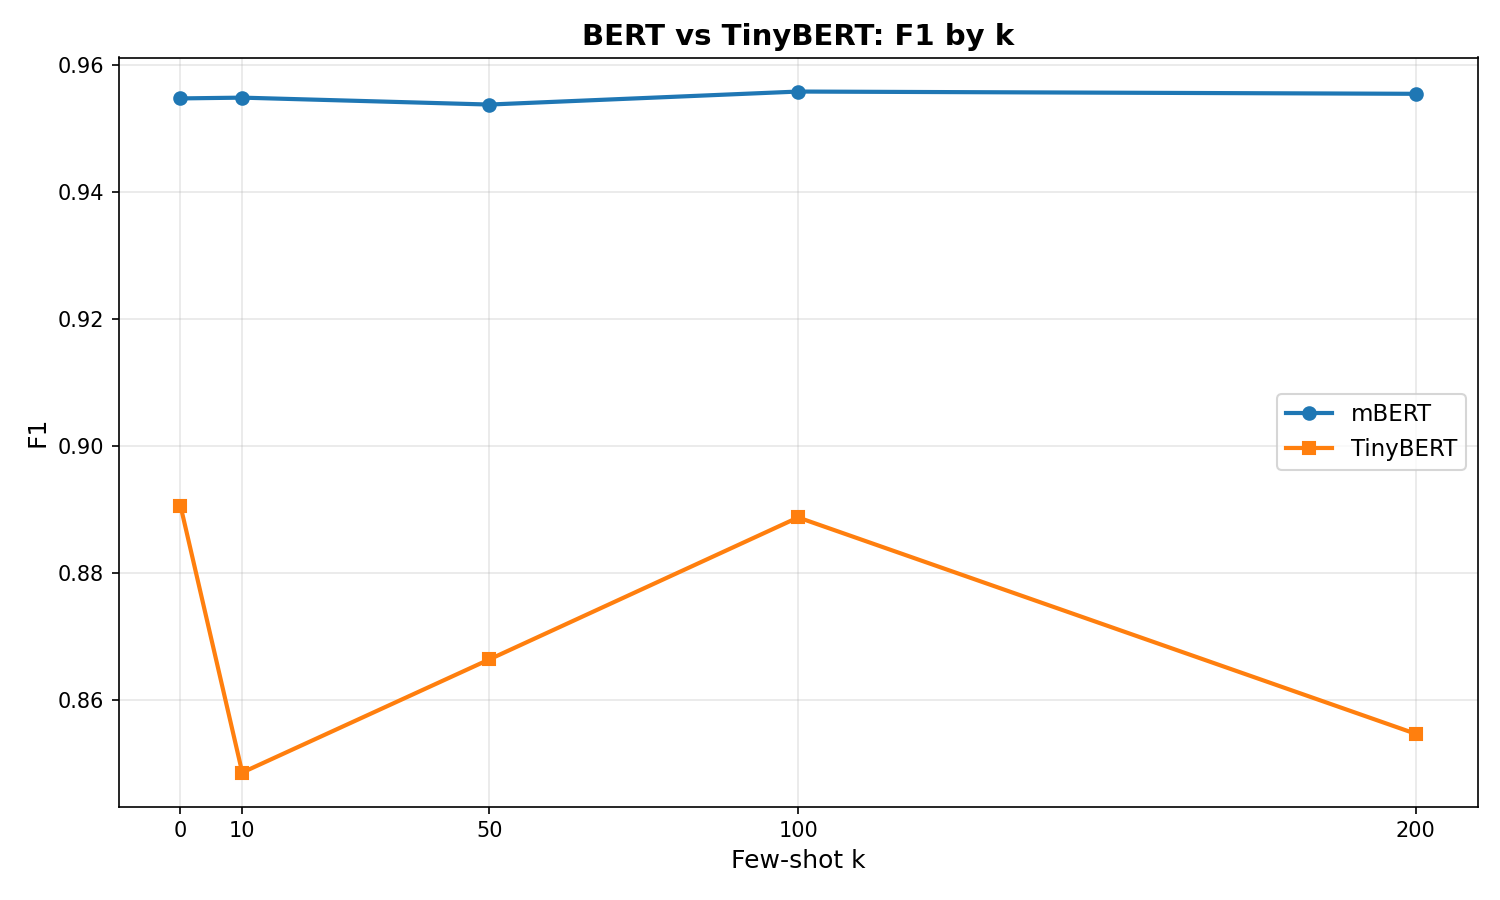
\includegraphics[width=0.95\columnwidth]{../code/graphs/bert_tinybert_k_comparison/bert_tinybert_f1.png}
\caption{Primerjava metrike F1 med mBERT in TinyBERT modelom glede na število few-shot primerov. mBERT je praktično nespremenjen pri vseh $k$, medtem ko je TinyBERT ne-monoton: pri $k=10$ in $k=200$ opazimo padec, najvišji rezultat pa doseže pri $k=0$ (zero-shot), zelo blizu pa je tudi pri $k=100$.}
\label{fig:bert_tinybert_comparison}
\end{figure}

\begin{figure}[!htbp]
\centering
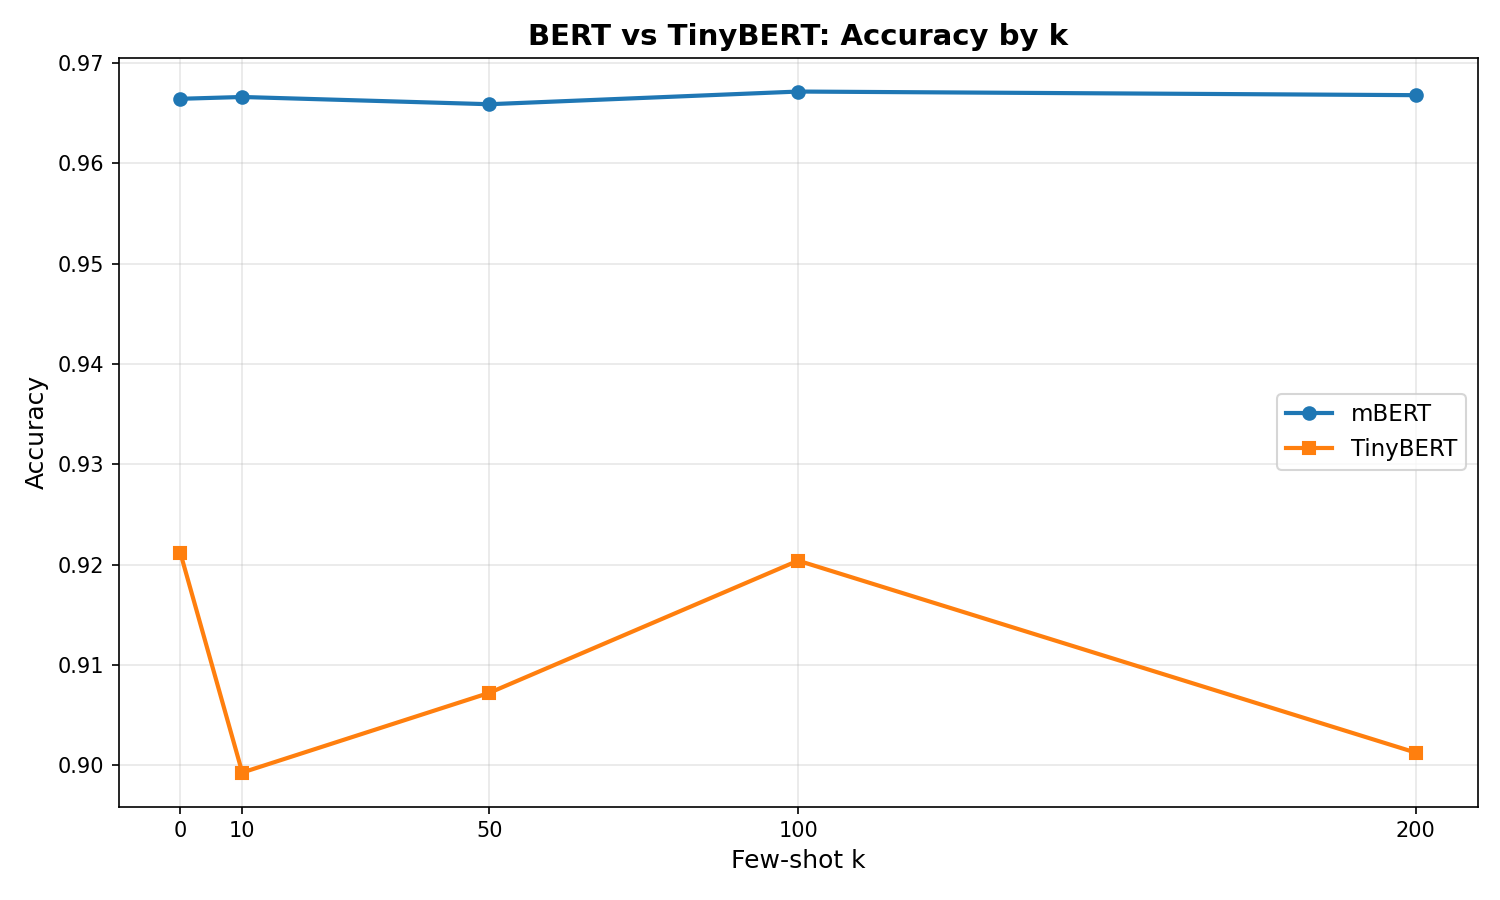
\includegraphics[width=0.95\columnwidth]{../code/graphs/bert_tinybert_k_comparison/bert_tinybert_accuracy.png}
\caption{Primerjava točnosti med mBERT in TinyBERT glede na število few-shot primerov. Ker je razred \textit{ham} pogostejši, ostane točnost visoka tudi pri scenarijih, kjer se priklic spama poslabša; zato je pri interpretaciji pomembno spremljati tudi priklic in F1.}
\label{fig:bert_tinybert_accuracy}
\end{figure}

\begin{figure}[!htbp]
\centering
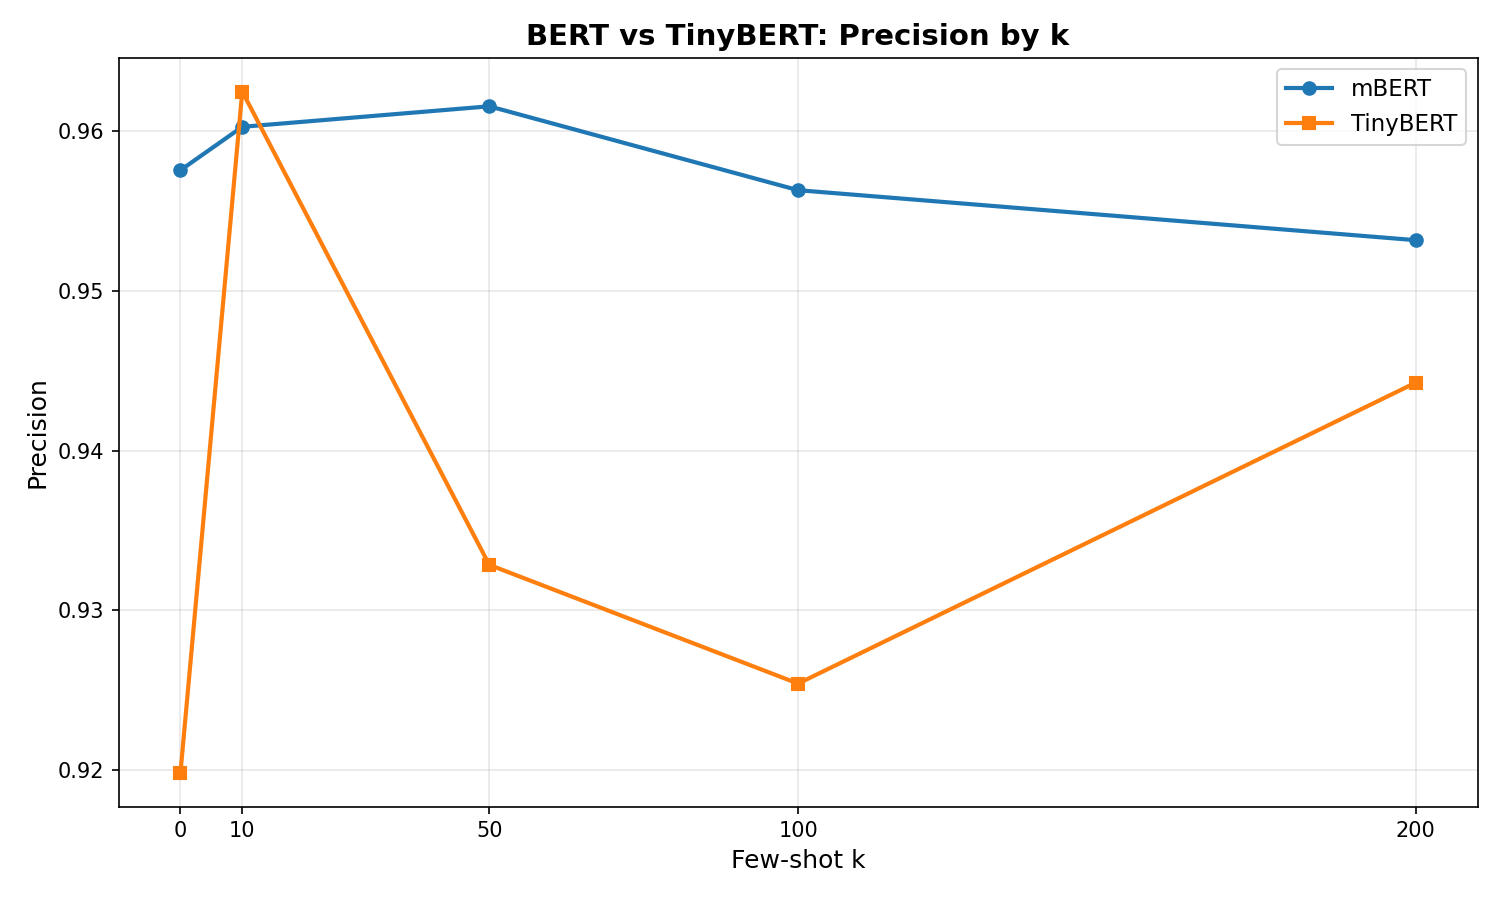
\includegraphics[width=0.95\columnwidth]{../code/graphs/bert_tinybert_k_comparison/bert_tinybert_precision.png}
\caption{Primerjava natančnosti med mBERT in TinyBERT glede na število few-shot primerov. Pri TinyBERT se natančnost pri nekaterih $k$ poveča (manj lažno pozitivnih), vendar to ne pomeni nujno boljšega F1, če se hkrati zmanjša priklic.}
\label{fig:bert_tinybert_precision}
\end{figure}

\begin{figure}[!htbp]
\centering
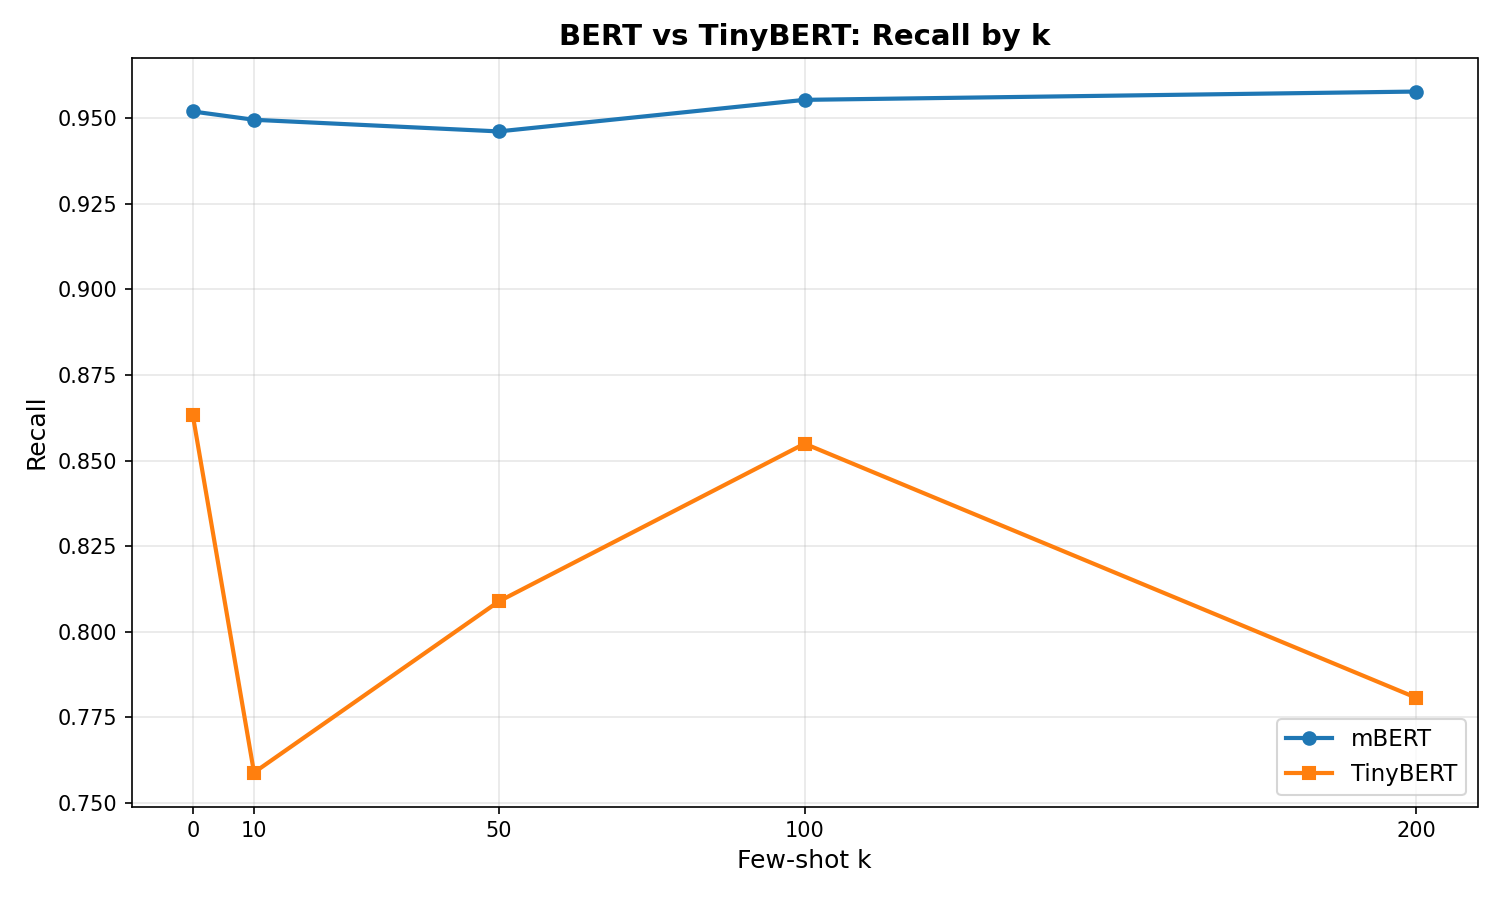
\includegraphics[width=0.95\columnwidth]{../code/graphs/bert_tinybert_k_comparison/bert_tinybert_recall.png}
\caption{Primerjava priklica med mBERT in TinyBERT glede na število few-shot primerov. Padec F1 pri TinyBERT pri $k=10$ in $k=200$ sovpada z opaznim padcem priklica (več zgrešenih \textit{spam} primerov), kar potrjuje, da je glavni problem pri teh $k$ povečanje lažno negativnih napovedi.}
\label{fig:bert_tinybert_recall}
\end{figure}

\subsubsection{Rezultati po vrednosti $k$}

Tabela~\ref{tab:per_k_comparison} prikazuje F1 vrednosti obeh modelov za različne nastavitve $k$.

\begin{table}[h]
\centering
\caption{F1 vrednosti mBERT in TinyBERT po vrednosti $k$.}
\label{tab:per_k_comparison}
\begin{tabular}{rccc}
\toprule
\textbf{k} & \textbf{mBERT F1} & \textbf{TinyBERT F1} & \textbf{F1 razlika} \\
\midrule
0 & 0,9547 & 0,8906 & 0,0641 \\
10 & 0,9549 & 0,8486 & 0,1063 \\
50 & 0,9538 & 0,8664 & 0,0874 \\
100 & 0,9558 & 0,8888 & 0,0670 \\
200 & 0,9555 & 0,8547 & 0,1008 \\
\bottomrule
\end{tabular}
\end{table}

Opažanja s primerjave:
\begin{itemize}
    \item mBERT dosega F1 vrednosti med 0,9538 in 0,9558 v vseh testiranih scenarijih.
    \item TinyBERT dosega nižje F1 vrednosti, v razponu med 0,8486 in 0,8906.
    \item Razlika v F1 med modeloma se giblje med 0,0641 (pri $k=0$) in 0,1063 (pri $k=10$).
    \item Pri $k=100$ je razlika najmanjša (0,0670), pri $k=10$ je največja (0,1063).
    \item Oba modela pri vrednostih $k=50$ in $k=100$ dosegata višji F1 kot pri $k=10$.
\end{itemize}

\subsubsection{Matrike zmede}

Za boljšo razlago razlik med natančnostjo in priklicem prikazujemo matrike zmede. V nadaljevanju interpretiramo predvsem \textit{FP} (Lažni pozitivi, ham $\rightarrow$ spam) in \textit{FN} (Lažni negativi, spam $\rightarrow$ ham), saj neposredno pojasnjujeta spremembe v natančnosti in priklicu.

\begin{figure}[!htbp]
\centering
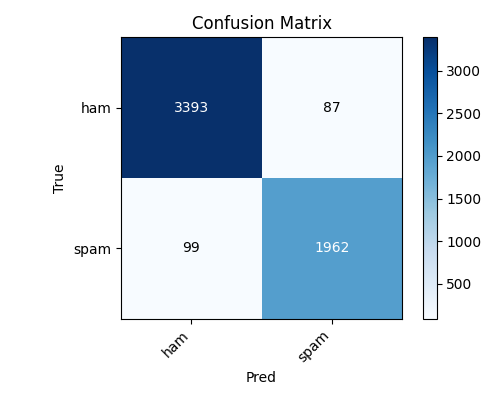
\includegraphics[width=0.90\columnwidth]{../code/graphs/bert-base-multilingual-cased_zero_shot_eval_2026-05-10_15-27-23/confusion_matrix.png}
\caption{Matrika zmede mBERT v zero-shot scenariju (EN $\rightarrow$ SL). Model naredi malo napak: $FP=87$ (ham označen kot spam) in $FN=99$ (spam označen kot ham), pri čemer sta tudi $TN=3393$ in $TP=1962$ visoka. To pomeni, da mBERT hkrati dobro zazna spam (nizek \textit{FN}) in ne ustvarja veliko lažnih alarmov (nizek \textit{FP}), zato sta natančnost in priklic visoka ter uravnotežena.}
\label{fig:cm_mbert_zero_shot}
\end{figure}

\begin{figure}[!htbp]
\centering
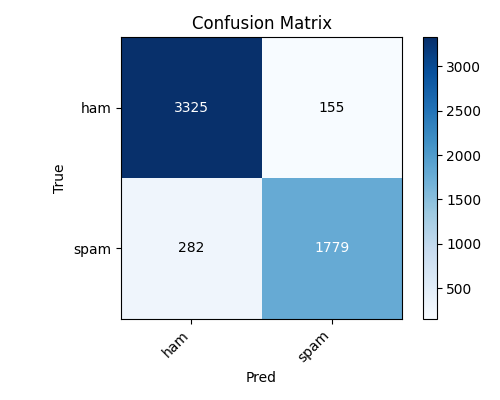
\includegraphics[width=0.90\columnwidth]{../code/graphs/TinyBERT_General_4L_312D_zero_shot_eval_2026-05-10_14-46-05/confusion_matrix.png}
\caption{Matrika zmede TinyBERT v zero-shot scenariju. V primerjavi z mBERT ima več napak: $FP=155$ in predvsem več lažno negativnih $FN=282$ (spam označen kot ham), kar pomeni, da model del spama \emph{spregleda}. To se neposredno vidi v nižjem priklicu (več zgrešenih spamov) in posledično nižjem F1, četudi je natančnost še vedno razmeroma visoka.}
\label{fig:cm_tinybert_zero_shot}
\end{figure}

\begin{figure}[!htbp]
\centering
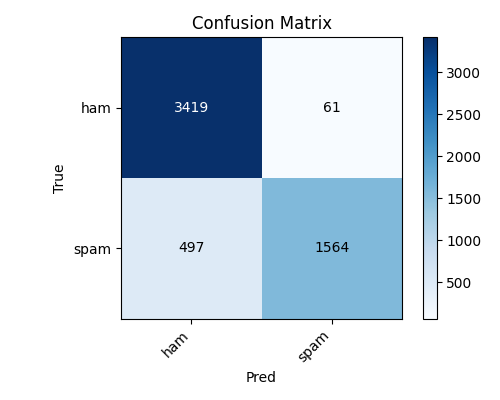
\includegraphics[width=0.90\columnwidth]{../code/graphs/TinyBERT_General_4L_312D_fewshot_k10_2026-05-10_14-47-27/confusion_matrix.png}
\caption{Matrika zmede TinyBERT pri few-shot $k=10$. Model postane \emph{konzervativen} pri označevanju spama: $FP=61$ je nizko (malo ham sporočil je napačno označenih kot spam), vendar močno naraste $FN=497$ (veliko spama je napačno označenega kot ham). Posledično priklic spama izrazito pade, kar pojasni tudi padec F1 pri $k=10$, kljub zelo visoki natančnosti.}
\label{fig:cm_tinybert_k10}
\end{figure}

\begin{figure}[!htbp]
\centering
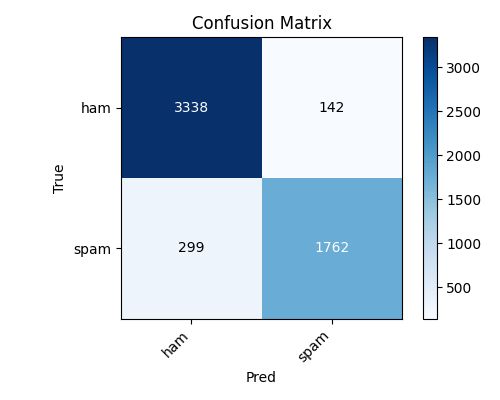
\includegraphics[width=0.90\columnwidth]{../code/graphs/TinyBERT_General_4L_312D_fewshot_k100_2026-05-10_14-50-22/confusion_matrix.png}
\caption{Matrika zmede TinyBERT pri few-shot $k=100$. V primerjavi s $k=10$ se ravnotežje izboljša: $FN$ pade na $299$, kar pomeni manj spregledanega spama in višji priklic, hkrati pa ostane $FP=142$ zmeren. Ta konfiguracija zato delno povrne izgubljeno učinkovitost glede na $k=10$ in se najbolj približa zero-shot rezultatu TinyBERT.}
\label{fig:cm_tinybert_k100}
\end{figure}

\begin{figure}[!htbp]
\centering
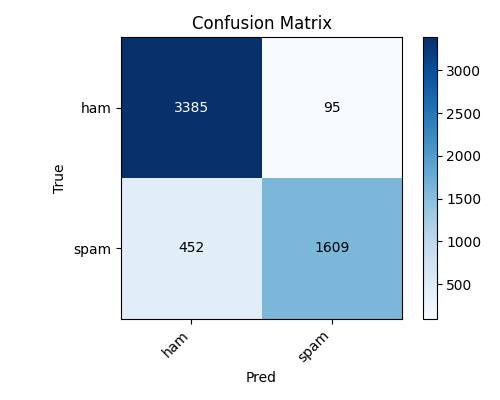
\includegraphics[width=0.90\columnwidth]{../code/graphs/TinyBERT_General_4L_312D_fewshot_k200_2026-05-10_14-52-05/confusion_matrix.png}
\caption{Matrika zmede TinyBERT pri few-shot $k=200$. Opazimo poslabšanje glede na $k=100$: $FN=452$ ponovno naraste (več spregledanega spama), $FP=95$ pa ostane relativno nizek. To kaže, da več slovenskih primerov v few-shot režimu ne prinese nujno stabilnejšega modela, temveč lahko potisne odločanje v smer, kjer model sicer ne dela veliko lažnih alarmov, a hkrati prepogosto spregleda spam, kar zniža F1.}
\label{fig:cm_tinybert_k200}
\end{figure}

\section{Diskusija}

Rezultati naših eksperimentov kažejo na več ključnih spoznanj o medjezikovnem prenosu znanja pri klasifikaciji SMS sporočil.

\subsection{Medjezikovni prenos znanja}

Primerjava zero-shot scenarijev (EN $\rightarrow$ SL) razkriva, da je mBERT model ohranil večino svoje zmogljivosti tudi pri testiranju na slovenščini. Čeprav je model naučen izključno na angleških podatkih, je dosegel F1 vrednost 0,9547 na slovenskem testnem naboru, kar je enako rezultatu na angleškem naboru (EN $\rightarrow$ EN). To kaže na izjemno sposobnost večjezikovnih modelov za semantičen prenos znanja med jeziki.

Nasprotno pa je TinyBERT pokazal znaten padec zmogljivosti pri medjezikovnem prenosu. Razlika v F1 vrednostih med mBERT in TinyBERT v zero-shot scenariju znaša 0,0641. Ta razlika je verjetno posledica manjše kapacitete modela in zmanjšane jezikovne reprezentacije, ki izhaja iz procesa destilacije znanja. Kljub temu je tudi TinyBERT ohranil sprejemljivo zmogljivost (F1 = 0,8906), kar je primerno za praktične aplikacije na mobilnih napravah.

\subsection{Vpliv few-shot prilagajanja}

Rezultati few-shot učenja kažejo zanimive vzorce. Pri mBERT modelu je dodatno fino prilagajanje s 10 do 200 primeri nekoliko izboljšalo ali ohranilo F1 vrednost. Razlike so majhne (v razponu 0,0011 do 0,0020), kar nakazuje, da je model že brez prilagajanja dosegel visoko generalizacijo.

Pri TinyBERT modelu pa vidimo bolj dinamičen odziv na few-shot učenje, pri katerem povečanje $k$ ne vodi v enolično izboljšanje (Slika~\ref{fig:bert_tinybert_comparison}). V našem primeru je izhodiščni zero-shot rezultat za TinyBERT visok (F1 = 0,8906), pri $k=10$ pa se učinkovitost občutno poslabša (F1 = 0,8486), nato se pri $k=50$ in $k=100$ delno povrne (F1 = 0,8664 in 0,8888), pri $k=200$ pa ponovno pade (F1 = 0,8547) (Tabela~\ref{tab:tinybert_fewshot}).

Grafi natančnosti in priklica (Sliki~\ref{fig:bert_tinybert_precision} in~\ref{fig:bert_tinybert_recall}) pokažejo, da je ta nihaj povezan s kompromisom med \emph{natančnostjo} in \emph{priklicem}. Pri $k=10$ TinyBERT doseže zelo visoko natančnost (0,9625), vendar hkrati močno pade priklic (0,7589), kar pomeni večje število lažno negativnih primerov spama; posledično pade tudi F1. Podobno pri $k=200$ natančnost ostane visoka (0,9442), priklic pa je nižji (0,7807), zato se F1 ne izboljša glede na izhodišče. Takšno obnašanje je skladno s scenarijem, kjer majhen in/ali domensko nehomogen nabor few-shot primerov povzroči nestabilno prilagajanje (prevelik vpliv posameznih primerov) in slabšo generalizacijo.

\subsection{Praktične implikacije}

Naši rezultati imajo jasne posledice za praktično uporabo:

\textbf{Za splošno uporabo:} mBERT je idealen izbor, saj dosega izjemno visoko zmogljivost brez potrebe po dodatnem učenju na ciljnem jeziku. Njegov zero-shot pristop je praktičen za hitro razporeditev v novih jezikih.

\textbf{Za mobilne naprave:} TinyBERT je primeren izbor za lokalno obdelavo na napravah z omejenimi viri. Čeprav je zmogljivost nižja, few-shot prilagajanje na 50--100 slovenskih primerih lahko delno povrne padec glede na $k=10$, vendar učinek ni stabilen in ne zagotavlja enoličnega približevanja mBERT-u (Slika~\ref{fig:bert_tinybert_comparison}). To je ključno za sisteme, ki potrebujejo visoko stopnjo zasebnosti in delovanje brez internetne povezave.

\textbf{Za jezikovne pare:} Angleščina-slovenščina se je izkazala za dovolj semantično povezana, da omogoči učinkovit medjezikovni prenos znanja. To nakazuje, da so drugi indoevropski jeziki, kot so španski, nemščina ali francosčina, verjetno enako ali še bolj primerni za take pristope.

\subsection{Omejitve raziskave}

Čeprav so rezultati obetavni, je treba opozoriti na nekaj omejitev:

\begin{itemize}
    \item \textbf{Velikost nabora:} Študija se osredotoča na slovenski testni nabor fiksne velikosti. Dodatne analize z različnimi velikostmi testnih naborov bi dale podrobnejši vpogled v generalizacijo.
    \item \textbf{Domenske razlike:} SMS sporočila v angleščini in slovenščini lahko vsebujejo različne vzorce spama, kar bi lahko vplivalo na rezultate.
    \item \textbf{Primerjava z drugimi pristopi:} Študija se osredotoča na transformatorske modele. Primerjava s klasičnimi metodami (SVM, logistična regresija) bi bila vredna za popolnejšo evalvacijo.
\end{itemize}

\section{Zaključek}

V članku smo obravnavali problem večjezične klasifikacije neželenih SMS sporočil s poudarkom na praktični uporabnosti v okoljih z omejenimi viri. Z uporabo strategij učenja brez primerov (zero-shot) in učenja z malo primeri (few-shot) smo primerjali večji model mBERT in bistveno manjši, mobilno usmerjen model TinyBERT na jezikovnem paru angleščina--slovenščina.

Rezultati potrjujejo, da mBERT izkazuje zelo stabilen medjezikovni prenos znanja: F1 na slovenskem testnem naboru v zero-shot scenariju ostane primerljiv z rezultatom v scenariju EN $\rightarrow$ EN, few-shot prilagajanje pa prinese le minimalne spremembe. To kaže, da lahko za zelo natančno detekcijo spama v slovenščini v praksi pogosto zadostuje že model, naučen na angleških podatkih.

Pri TinyBERT smo opazili drugačen vzorec. V zero-shot scenariju je zmogljivost nižja kot pri mBERT, few-shot prilagajanje pa se je izkazalo kot občutljivo na izbiro velikosti nabora $k$. V naših eksperimentih povečanje števila slovenskih primerov ni vodilo v enolično izboljševanje, temveč se je pri večjem številu primerov začela zmogljivost tudi slabšati (npr. pri $k=200$ je F1 nižji kot pri $k=0$ in $k=100$). To nakazuje, da pri manjših modelih zgolj dodajanje več primerov brez dodatne prilagoditve učnih nastavitev (npr. število epoh, regularizacija, zgodnje ustavljanje) lahko privede do nestabilnega prilagajanja in slabše generalizacije.

Sklepno ugotavljamo, da je mBERT primernejša izbira, kadar je prioritetna najvišja klasifikacijska zmogljivost in je na voljo dovolj računske moči, medtem ko TinyBERT ostaja smiseln kandidat za mobilne naprave, kjer je ključna majhnost modela, a zahteva bolj previdno prilagoditev in validacijo na ciljnem jeziku. V prihodnje bi bilo smiselno preveriti vpliv različnih učnih hiperparametrov za TinyBERT v few-shot režimu, vključiti dodatne klasične baseline pristope (npr. SVM) ter razširiti evalvacijo na več slovenskih podatkovnih virov in domenskih variacij.


\bibliographystyle{ACM-Reference-Format}
\bibliography{bibliografija}

\end{document}